\chapter{Evolutionary Methods }
\label{chap:evo}

\section{Evolutionary Algorithms}

\todo{GA principles: loop / 1+lambda}

\section{Evolution of policies}

\todo{Evolutionary Programming / Genetic Programming (CGP) / ERL}

\section{NeuroEvolution}
\subsection{Direct encoding}
The first approach relies on directly encoding the final neural network, used to choose an action during the game, as an individual for the genetic algorithm. Each weight is therefore directly mutated by the algorithm.

\subsubsection{Weight Evolution with Evolution Strategies}
Similarly to a gradient-based methods, this technique aims to optimize synaptic weights and biases in a neural network by using evolutionary algorithms such as Covariance Matrix Adaptation Evolution Strategy (CMA-ES). \cite{CMA-ES} \cite{CMAES-Atari}\\ 
CMA-ES is a population-based stochastic derivative-free method that creates new populations based on a distribution, which evolves from the distribution in the previous generation based on which candidates performed best (Fig. \ref{CMA-ES}).

\begin{figure}[H]
 \centering
 \captionsetup{justification=centering, margin=0.5cm}
 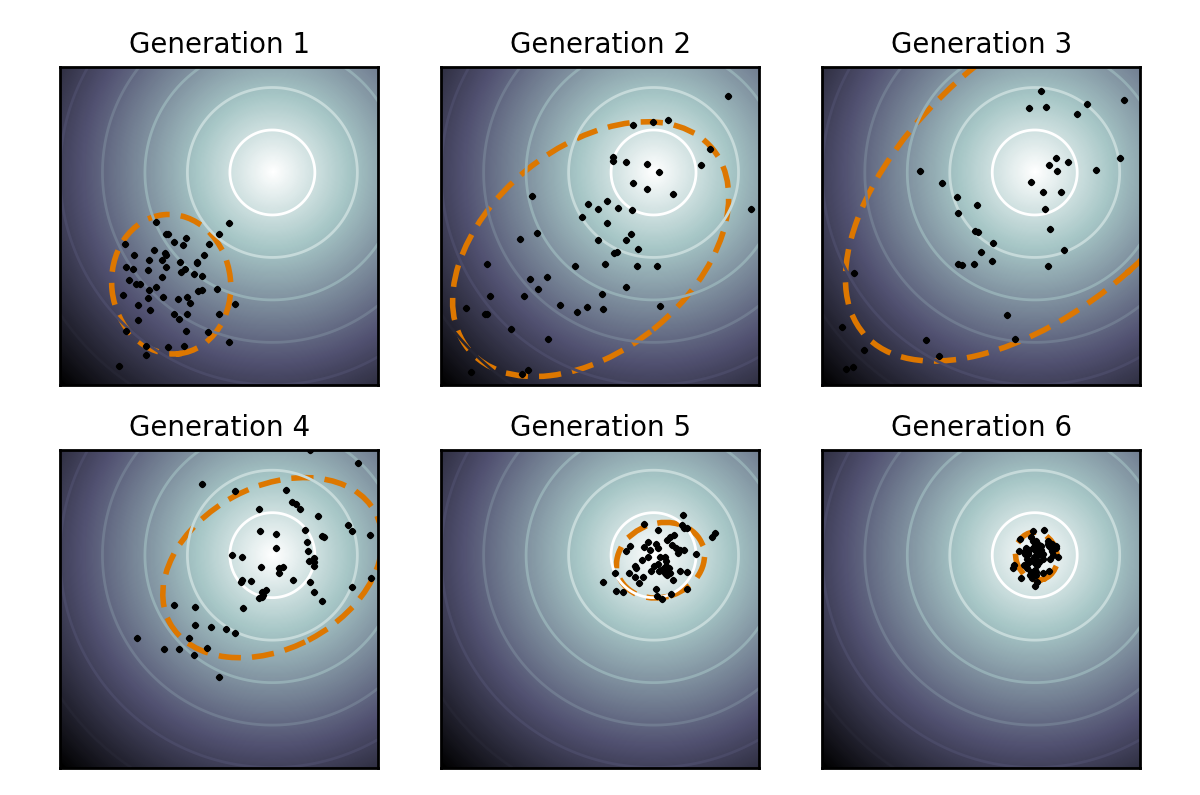
\includegraphics[width=7cm]{images/CMA_ES.png}
 \caption{\label{CMA-ES}Illustration of an actual optimization run with CMA-ES on a simple two-dimensional problem. The spherical optimization landscape is depicted with solid lines of equal-values. The population (dots) is much larger than necessary, but clearly shows how the distribution of the population (dotted line) changes during the optimization.}
\small\textsuperscript{\url{https://en.wikipedia.org/wiki/CMA-ES#/media/File:Concept_of_directional_optimization_in_CMA-ES_algorithm.png}}
 \label{CMA-ES}
\end{figure}

\bigbreak

\subsubsection{NEAT}
Since the architecture of a neural network (e.g. number of layers, size of each layer, recurrent units) can have a strong impact on final performance, this technique evolves both network structure and neuron weights on the final network. The NeuroEvolution of Augmenting Topologies algorithm (NEAT) created in 2002 (\cite{NEAT_1, NEAT_2}) presents solutions to 3 fundamental issues in the evolution of neural networks:

\begin{itemize}
    \item \textbf{Crossover between different structures}: NEAT provides a genotype-to-phenotype mapping based on mutations (Fig. \ref{NEAT}).
    \item \textbf{Protection of topological innovation}: The speciation mechanism evaluates candidates by comparing them to similar architectures to allow new structures to mature without being instantly eliminated. 
    \item \textbf{Minimization of structural complexity}: Nodes are added to a minimal initial structure in order to prevent networks from being too big without benefits.
\end{itemize}
\bigbreak

Multiple variants have been created from NEAT, including rtNEAT \cite{rtNEAT} for real-time neuroevolution, FS-NEAT \cite{FS-NEAT} for feature selection, or HyperNeat based on indirect encoding \cite{HyperNEAT}.

\begin{figure}[H]
 \centering
 \captionsetup{justification=centering, margin=0.5cm}
 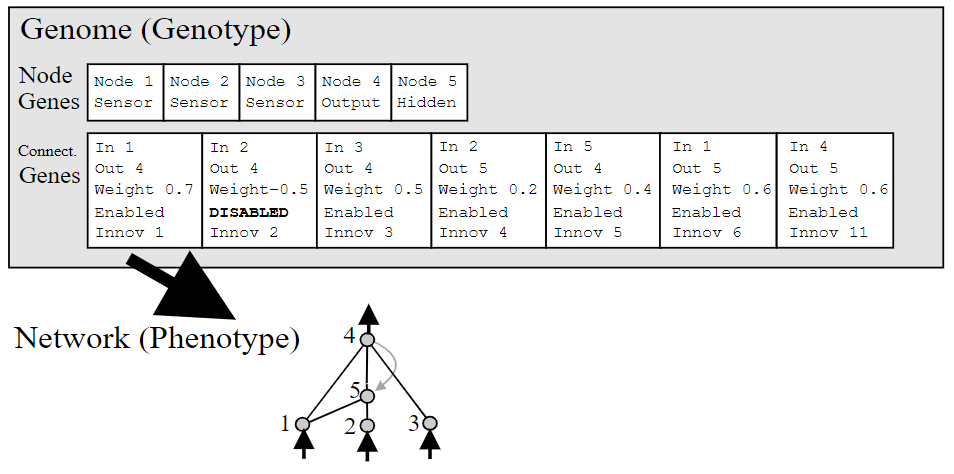
\includegraphics[width=7cm]{images/neat.png}
 \caption{\label{NEAT}NEAT genotype-to-phenotype mapping example. A genotype is depicted that produces the shown phenotype. There are 3 input nodes, one hidden, and one output node, and seven connection definitions, one of which is recurrent. \cite{NEAT_2}}
 \label{fig:NEAT}
\end{figure}

A deeper description of NEAT is introduced in chapter \ref{chap:neuroevo}.

\subsection{Indirect encoding}
Goal: reuse the same information multiple time, reduce the search space to a more efficient one
Principle: encode the weights of a NN with an evolved program

The second approach uses an intermediary program, optimized through an evolutionary algorithm, to generate the synaptic weights of the final neural network based on their positions. 

HyperNEAT \cite{HyperNEAT} uses a Compositional Pattern Producing Network (CPPN) \cite{CPPN} optimized through a NEAT-based process to create the final network. This allows the final network to be larger without increasing the size of the space to explore, since the same CPPN can be used on any number of neurons.

As Compositional Pattern Producing Networks implement multiple activation functions including Gaussian, sigmoid, and periodic functions, they can produce connectivity patterns with symmetries based on the positions of the neurons, better exploiting regularities in the task.

\section{Quality Diversity approaches}

\section{Coevolution}

%%% Local Variables: 
%%% mode: latex
%%% TeX-master: "isae-report-template"
%%% End: 